\documentclass[12pt]{article}
\usepackage[table]{xcolor}
\usepackage[shortlabels]{enumitem}
\usepackage{tabularx,xltabular}
\usepackage{graphicx}
\usepackage{hyperref}
\usepackage{verbatim}
\usepackage{geometry}
\usepackage{ulem}
\usepackage[official]{eurosym}
\usepackage{tikz}
\usetikzlibrary{arrows,backgrounds,calc,decorations.markings,patterns,3d}
\usepackage{pgfplots}
\pgfplotsset{compat = newest}
\usetikzlibrary{fit}
\newcommand\addvmargin[1]{
\usetikzlibrary{arrows}
\node[fit=(current bounding box),inner ysep=#1,inner xsep=0]{};}
\usepackage{cancel}
\usepackage{fontspec}
\usepackage{array}  
\geometry{a4paper, top=2cm, left=2cm, right=2cm, bottom=2cm, headsep=1cm}
\usepackage{tabu}
\usepackage{pst-node}
\usepackage{colortbl}
\usepackage{array}
\usepackage{german}
\setlength\parindent{0pt}
\newcolumntype{?}{!{\vrule width 1pt}}
\usepackage{makecell}
\renewcommand{\arraystretch}{2.5}
\usepackage{pbox}
\usepackage{amssymb}
\usepackage{amsmath}
\usepackage{booktabs}
\newcolumntype{L}[1]{>{\raggedright\let\newline\\\arraybackslash\hspace{0pt}}m{#1}}
\newcolumntype{C}[1]{>{\centering\let\newline\\\arraybackslash\hspace{0pt}}m{#1}}
\newcolumntype{R}[1]{>{\raggedleft\let\newline\\\arraybackslash\hspace{0pt}}m{#1}}
\begin{document}
\rightline{Datum: 14.06.2023}
\centerline{{\Large Terme und Gleichungen}} 
\vspace{1cm}
\noindent \\


\begin{xltabular}{\textwidth}{|C{0.75cm}|X|C{0.75cm}|X|}
\arrayrulecolor{black}\hline
a)&Setze für die Variabel a den Wert -8 ein und berechne den Wert des Terms:$$5 \cdot a + 5 \cdot a$$
&
b)&Setze für die Variabel x den Wert -12 ein und berechne den Wert des Terms:$$x - 1$$
\\\hline
c)&Setze für die Variabel x den Wert -5 ein und berechne den Wert des Terms:$$4 \cdot x + 1$$
&
d)&Setze für die Variabel z den Wert 7 ein und berechne den Wert des Terms:$$z + 4$$
\\\hline
e)&Bestimme ein Term, wenn x=5 und das Ergebnis gleich 10 ist.
&
f)&Bestimme ein Term, wenn x=6 und das Ergebnis gleich 36 ist.
\\\hline
g)&Bestimme ein Term, wenn x=10 und das Ergebnis gleich 0 ist.
&
h)&Bestimme ein Term, wenn x=3 und das Ergebnis gleich 0 ist.
\\\hline
i)&Vereinfache:$$1 + y - 2$$
&
j)&Vereinfache:$$5 - 5 \cdot y - 4 \cdot y$$
\\\hline
k)&Vereinfache:$$4 \cdot b + 3 \cdot b - 1$$
&
l)&Vereinfache:$$3 \cdot a + a + 3$$
\\\hline
m)&Berechne die Variable $$-10-3-4\cdot x+9\cdot x=12$$
&
n)&Berechne die Variable $$-6\cdot y+13\cdot y-4-11=13$$
\\\hline
o)&Berechne die Variable $$2-3\cdot x-6+11\cdot x=68$$
&
p)&Berechne die Variable $$-23-4\cdot b+13\cdot b+9=49$$
\\\hline
q)&Berechne die Variable $$5\cdot a+2-5+1\cdot a=27$$
&
r)&Berechne die Variable $$-31+15+4\cdot y+3\cdot y=68$$
\\\hline
s)&Berechne die Variable $$-21+2\cdot a+7+1\cdot a=1$$
&
t)&Berechne die Variable $$-8+1\cdot y-2+4\cdot y=0$$
\\\hline
u)&Berechne die Variable $$3\cdot x+6\cdot x-27+13=85$$
&
v)&Berechne die Variable $$-6-9-4\cdot x+9\cdot x=30$$
\\\hline
w)&Berechne die Variable $$2+1\cdot b+3\cdot b-21=1$$
&
x)&Berechne die Variable $$2\cdot x-4+6\cdot x-7=53$$
\\\hline
y)&Berechne die Variable $$-4+3\cdot b-3+7\cdot b=93$$
&
z)&Berechne die Variable $$5\cdot b-13-6-1\cdot b=29$$
\\\hline
\end{xltabular}
\vspace{0.5cm}
\newpage
\rightline{Datum: 14.06.2023}
\centerline{{\large Lösungen Terme und Gleichungen}} 
\vspace{0.5cm}

\begin{xltabular}{\textwidth}{|C{0.75cm}|X|C{0.75cm}|X|}
\arrayrulecolor{black}\hline
a)&$\begin{aligned}
\textcolor{red}{a=-8} & \rightarrow\\
5 \cdot a + 5 \cdot a=&5 \cdot \textcolor{red}{(-8)} + 5 \cdot \textcolor{red}{(-8)}=-80\\
\end{aligned}$
&
b)&$\begin{aligned}
\textcolor{red}{x=-12} & \rightarrow\\
x - 1=&\textcolor{red}{(-12)} - 1=-13\\
\end{aligned}$
\\\hline
c)&$\begin{aligned}
\textcolor{red}{x=-5} & \rightarrow\\
4 \cdot x + 1=&4 \cdot \textcolor{red}{(-5)} + 1=-19\\
\end{aligned}$
&
d)&$\begin{aligned}
\textcolor{red}{z=7} & \rightarrow\\
z + 4=&\textcolor{red}{7} + 4=11\\
\end{aligned}$
\\\hline
e)&Ein mögliches Ergebnis:\[ x=5 ~~ \rightarrow x+5=10 \]
&
f)&Ein mögliches Ergebnis:\[ x=6 ~~ \rightarrow x \cdot 6=36 \]
\\\hline
g)&Ein mögliches Ergebnis:\[ x=10 ~~ \rightarrow x-10=0 \]
&
h)&Ein mögliches Ergebnis:\[ x=3 ~~ \rightarrow x-3=0 \]
\\\hline
i)&$1 + y - 2=y - 1$
&
j)&$5 - 5\cdot y - 4\cdot y=5 - 9y$
\\\hline
k)&$4\cdot b + 3\cdot b - 1=7b - 1$
&
l)&$3\cdot a + a + 3=4a + 3$
\\\hline
m)&\begingroup\setlength{\jot}{-0.03cm}
\tikzstyle{background grid}=[draw, black!15,step=.5cm]
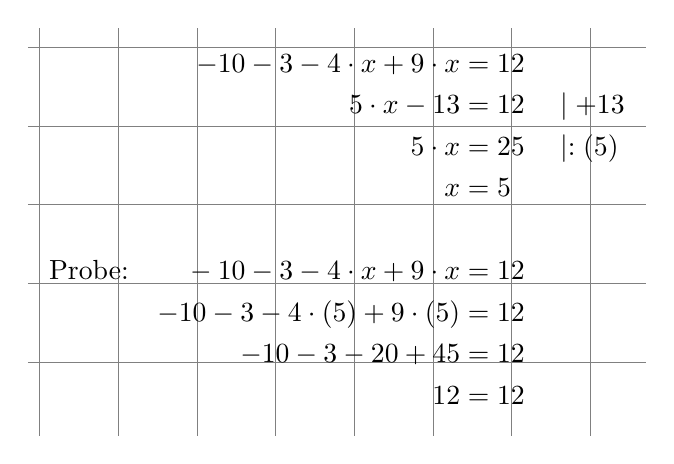
\begin{tikzpicture}[show background grid]
\node[below right] at (0,0.1) {
$\begin{aligned}
-10-3-4\cdot x+9\cdot x &=12& &  \\
5\cdot x - 13 &=12& & \mid + 13\\
5\cdot x &=25& & \mid :\left(5\right)\\
x &=5& & 
\\
\\
\mbox{Probe:}\qquad -10-3-4\cdot x+9\cdot x &=12& &  \\
-10-3-4\cdot \left(5\right)+9\cdot \left(5\right) &=12& &  \\
-10-3-20+45 &=12& &  \\
12 &=12& &  \\
\end{aligned}$};
\end{tikzpicture}
\endgroup
&
n)&\begingroup\setlength{\jot}{-0.03cm}
\tikzstyle{background grid}=[draw, black!15,step=.5cm]
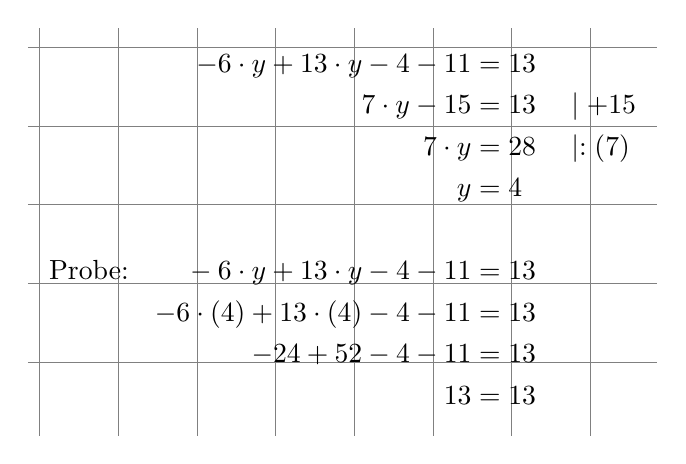
\begin{tikzpicture}[show background grid]
\node[below right] at (0,0.1) {
$\begin{aligned}
-6\cdot y+13\cdot y-4-11 &=13& &  \\
7\cdot y - 15 &=13& & \mid + 15\\
7\cdot y &=28& & \mid :\left(7\right)\\
y &=4& & 
\\
\\
\mbox{Probe:}\qquad -6\cdot y+13\cdot y-4-11 &=13& &  \\
-6\cdot \left(4\right)+13\cdot \left(4\right)-4-11 &=13& &  \\
-24+52-4-11 &=13& &  \\
13 &=13& &  \\
\end{aligned}$};
\end{tikzpicture}
\endgroup
\\\hline
o)&\begingroup\setlength{\jot}{-0.03cm}
\tikzstyle{background grid}=[draw, black!15,step=.5cm]
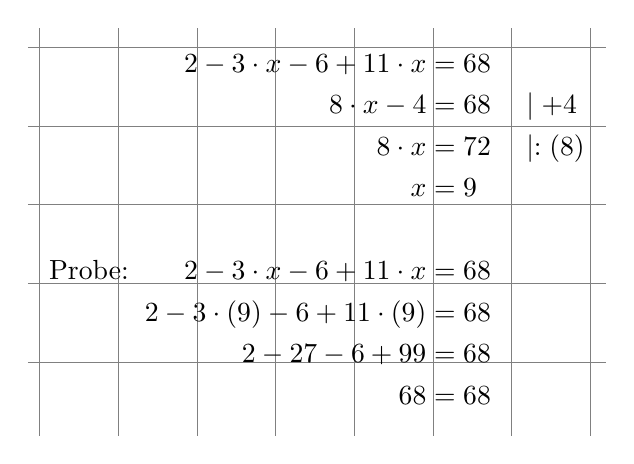
\begin{tikzpicture}[show background grid]
\node[below right] at (0,0.1) {
$\begin{aligned}
2-3\cdot x-6+11\cdot x &=68& &  \\
8\cdot x - 4 &=68& & \mid + 4\\
8\cdot x &=72& & \mid :\left(8\right)\\
x &=9& & 
\\
\\
\mbox{Probe:}\qquad 2-3\cdot x-6+11\cdot x &=68& &  \\
2-3\cdot \left(9\right)-6+11\cdot \left(9\right) &=68& &  \\
2-27-6+99 &=68& &  \\
68 &=68& &  \\
\end{aligned}$};
\end{tikzpicture}
\endgroup
&
p)&\begingroup\setlength{\jot}{-0.03cm}
\tikzstyle{background grid}=[draw, black!15,step=.5cm]
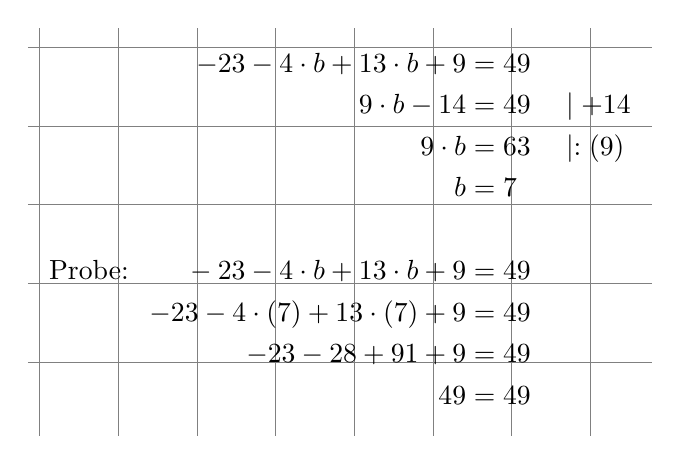
\begin{tikzpicture}[show background grid]
\node[below right] at (0,0.1) {
$\begin{aligned}
-23-4\cdot b+13\cdot b+9 &=49& &  \\
9\cdot b - 14 &=49& & \mid + 14\\
9\cdot b &=63& & \mid :\left(9\right)\\
b &=7& & 
\\
\\
\mbox{Probe:}\qquad -23-4\cdot b+13\cdot b+9 &=49& &  \\
-23-4\cdot \left(7\right)+13\cdot \left(7\right)+9 &=49& &  \\
-23-28+91+9 &=49& &  \\
49 &=49& &  \\
\end{aligned}$};
\end{tikzpicture}
\endgroup
\\\hline
q)&\begingroup\setlength{\jot}{-0.03cm}
\tikzstyle{background grid}=[draw, black!15,step=.5cm]
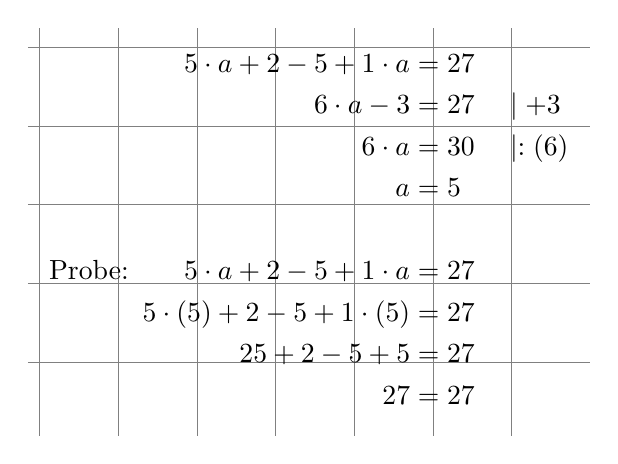
\begin{tikzpicture}[show background grid]
\node[below right] at (0,0.1) {
$\begin{aligned}
5\cdot a+2-5+1\cdot a &=27& &  \\
6\cdot a - 3 &=27& & \mid + 3\\
6\cdot a &=30& & \mid :\left(6\right)\\
a &=5& & 
\\
\\
\mbox{Probe:}\qquad 5\cdot a+2-5+1\cdot a &=27& &  \\
5\cdot \left(5\right)+2-5+1\cdot \left(5\right) &=27& &  \\
25+2-5+5 &=27& &  \\
27 &=27& &  \\
\end{aligned}$};
\end{tikzpicture}
\endgroup
&
r)&\begingroup\setlength{\jot}{-0.03cm}
\tikzstyle{background grid}=[draw, black!15,step=.5cm]
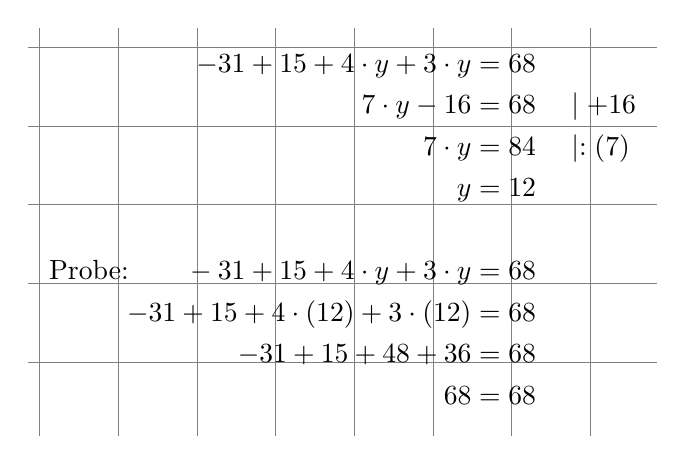
\begin{tikzpicture}[show background grid]
\node[below right] at (0,0.1) {
$\begin{aligned}
-31+15+4\cdot y+3\cdot y &=68& &  \\
7\cdot y - 16 &=68& & \mid + 16\\
7\cdot y &=84& & \mid :\left(7\right)\\
y &=12& & 
\\
\\
\mbox{Probe:}\qquad -31+15+4\cdot y+3\cdot y &=68& &  \\
-31+15+4\cdot \left(12\right)+3\cdot \left(12\right) &=68& &  \\
-31+15+48+36 &=68& &  \\
68 &=68& &  \\
\end{aligned}$};
\end{tikzpicture}
\endgroup
\\\hline
s)&\begingroup\setlength{\jot}{-0.03cm}
\tikzstyle{background grid}=[draw, black!15,step=.5cm]
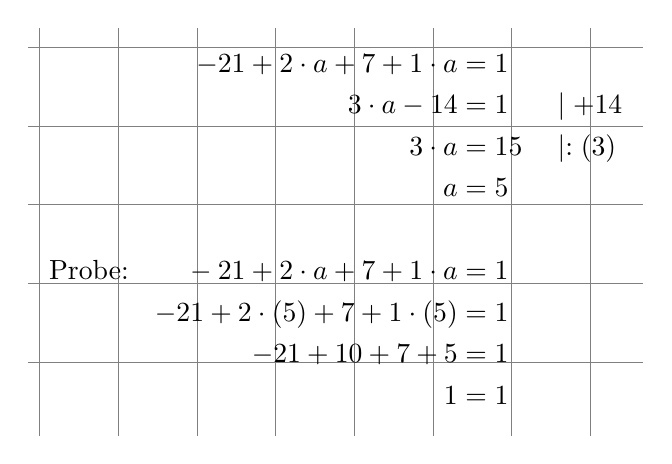
\begin{tikzpicture}[show background grid]
\node[below right] at (0,0.1) {
$\begin{aligned}
-21+2\cdot a+7+1\cdot a &=1& &  \\
3\cdot a - 14 &=1& & \mid + 14\\
3\cdot a &=15& & \mid :\left(3\right)\\
a &=5& & 
\\
\\
\mbox{Probe:}\qquad -21+2\cdot a+7+1\cdot a &=1& &  \\
-21+2\cdot \left(5\right)+7+1\cdot \left(5\right) &=1& &  \\
-21+10+7+5 &=1& &  \\
1 &=1& &  \\
\end{aligned}$};
\end{tikzpicture}
\endgroup
&
t)&\begingroup\setlength{\jot}{-0.03cm}
\tikzstyle{background grid}=[draw, black!15,step=.5cm]
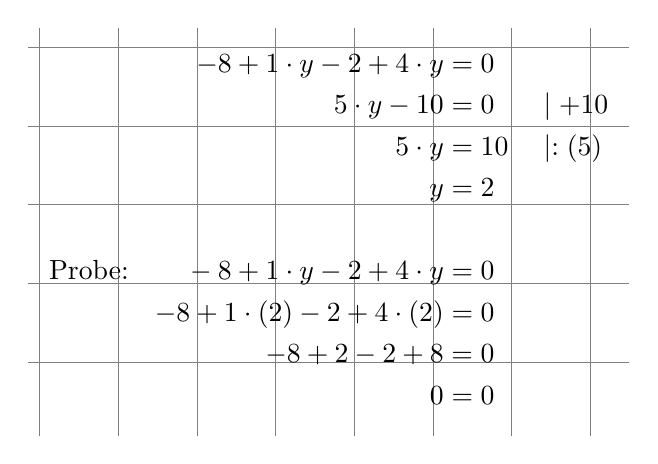
\begin{tikzpicture}[show background grid]
\node[below right] at (0,0.1) {
$\begin{aligned}
-8+1\cdot y-2+4\cdot y &=0& &  \\
5\cdot y - 10 &=0& & \mid + 10\\
5\cdot y &=10& & \mid :\left(5\right)\\
y &=2& & 
\\
\\
\mbox{Probe:}\qquad -8+1\cdot y-2+4\cdot y &=0& &  \\
-8+1\cdot \left(2\right)-2+4\cdot \left(2\right) &=0& &  \\
-8+2-2+8 &=0& &  \\
0 &=0& &  \\
\end{aligned}$};
\end{tikzpicture}
\endgroup
\\\hline
u)&\begingroup\setlength{\jot}{-0.03cm}
\tikzstyle{background grid}=[draw, black!15,step=.5cm]
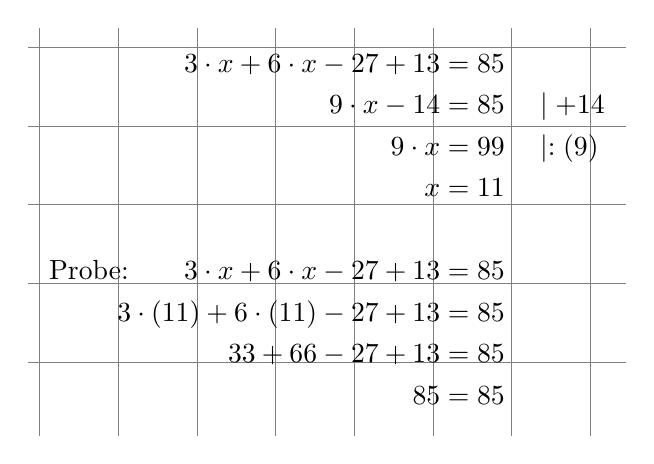
\begin{tikzpicture}[show background grid]
\node[below right] at (0,0.1) {
$\begin{aligned}
3\cdot x+6\cdot x-27+13 &=85& &  \\
9\cdot x - 14 &=85& & \mid + 14\\
9\cdot x &=99& & \mid :\left(9\right)\\
x &=11& & 
\\
\\
\mbox{Probe:}\qquad 3\cdot x+6\cdot x-27+13 &=85& &  \\
3\cdot \left(11\right)+6\cdot \left(11\right)-27+13 &=85& &  \\
33+66-27+13 &=85& &  \\
85 &=85& &  \\
\end{aligned}$};
\end{tikzpicture}
\endgroup
&
v)&\begingroup\setlength{\jot}{-0.03cm}
\tikzstyle{background grid}=[draw, black!15,step=.5cm]
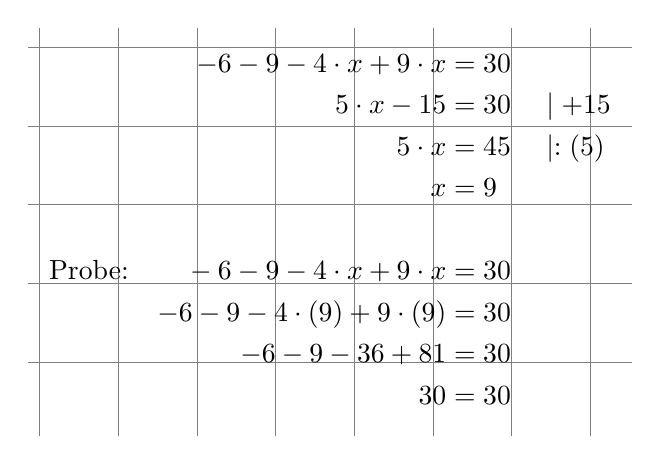
\begin{tikzpicture}[show background grid]
\node[below right] at (0,0.1) {
$\begin{aligned}
-6-9-4\cdot x+9\cdot x &=30& &  \\
5\cdot x - 15 &=30& & \mid + 15\\
5\cdot x &=45& & \mid :\left(5\right)\\
x &=9& & 
\\
\\
\mbox{Probe:}\qquad -6-9-4\cdot x+9\cdot x &=30& &  \\
-6-9-4\cdot \left(9\right)+9\cdot \left(9\right) &=30& &  \\
-6-9-36+81 &=30& &  \\
30 &=30& &  \\
\end{aligned}$};
\end{tikzpicture}
\endgroup
\\\hline
w)&\begingroup\setlength{\jot}{-0.03cm}
\tikzstyle{background grid}=[draw, black!15,step=.5cm]
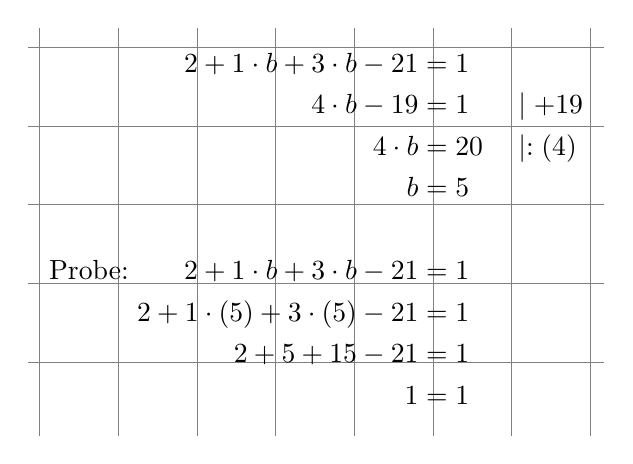
\begin{tikzpicture}[show background grid]
\node[below right] at (0,0.1) {
$\begin{aligned}
2+1\cdot b+3\cdot b-21 &=1& &  \\
4\cdot b - 19 &=1& & \mid + 19\\
4\cdot b &=20& & \mid :\left(4\right)\\
b &=5& & 
\\
\\
\mbox{Probe:}\qquad 2+1\cdot b+3\cdot b-21 &=1& &  \\
2+1\cdot \left(5\right)+3\cdot \left(5\right)-21 &=1& &  \\
2+5+15-21 &=1& &  \\
1 &=1& &  \\
\end{aligned}$};
\end{tikzpicture}
\endgroup
&
x)&\begingroup\setlength{\jot}{-0.03cm}
\tikzstyle{background grid}=[draw, black!15,step=.5cm]
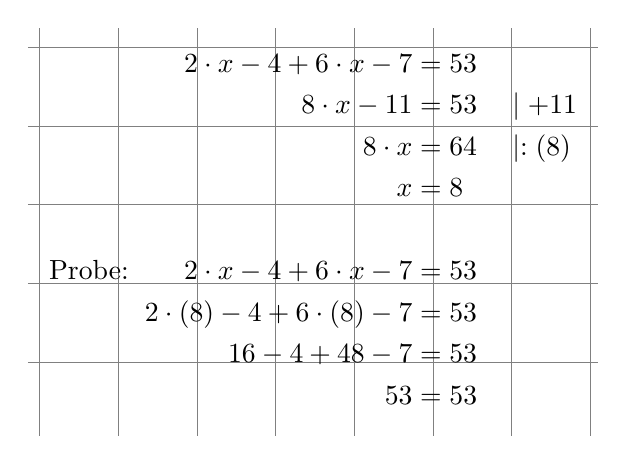
\begin{tikzpicture}[show background grid]
\node[below right] at (0,0.1) {
$\begin{aligned}
2\cdot x-4+6\cdot x-7 &=53& &  \\
8\cdot x - 11 &=53& & \mid + 11\\
8\cdot x &=64& & \mid :\left(8\right)\\
x &=8& & 
\\
\\
\mbox{Probe:}\qquad 2\cdot x-4+6\cdot x-7 &=53& &  \\
2\cdot \left(8\right)-4+6\cdot \left(8\right)-7 &=53& &  \\
16-4+48-7 &=53& &  \\
53 &=53& &  \\
\end{aligned}$};
\end{tikzpicture}
\endgroup
\\\hline
y)&\begingroup\setlength{\jot}{-0.03cm}
\tikzstyle{background grid}=[draw, black!15,step=.5cm]
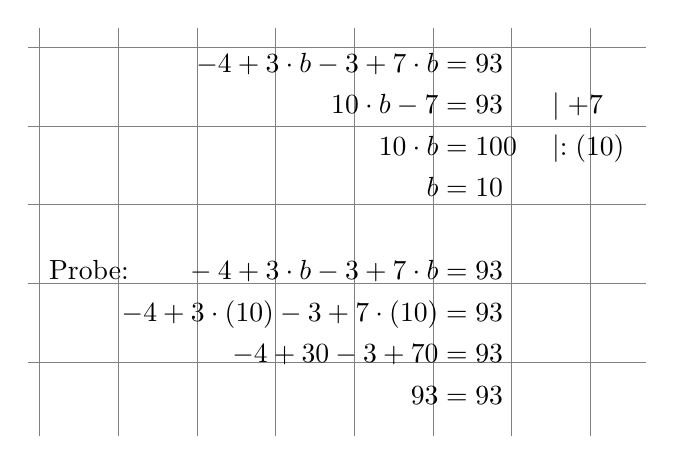
\begin{tikzpicture}[show background grid]
\node[below right] at (0,0.1) {
$\begin{aligned}
-4+3\cdot b-3+7\cdot b &=93& &  \\
10\cdot b - 7 &=93& & \mid + 7\\
10\cdot b &=100& & \mid :\left(10\right)\\
b &=10& & 
\\
\\
\mbox{Probe:}\qquad -4+3\cdot b-3+7\cdot b &=93& &  \\
-4+3\cdot \left(10\right)-3+7\cdot \left(10\right) &=93& &  \\
-4+30-3+70 &=93& &  \\
93 &=93& &  \\
\end{aligned}$};
\end{tikzpicture}
\endgroup
&
z)&\begingroup\setlength{\jot}{-0.03cm}
\tikzstyle{background grid}=[draw, black!15,step=.5cm]
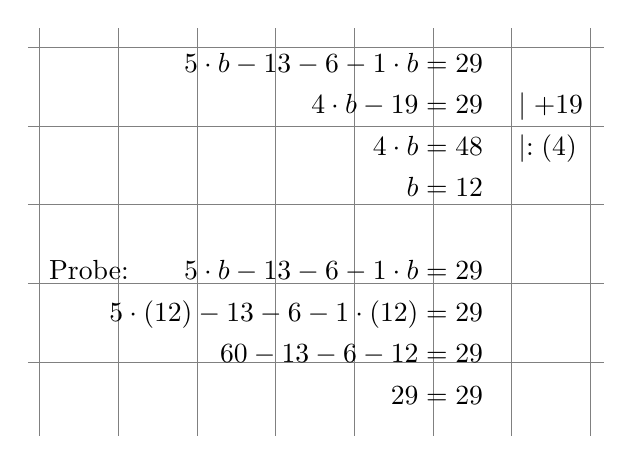
\begin{tikzpicture}[show background grid]
\node[below right] at (0,0.1) {
$\begin{aligned}
5\cdot b-13-6-1\cdot b &=29& &  \\
4\cdot b - 19 &=29& & \mid + 19\\
4\cdot b &=48& & \mid :\left(4\right)\\
b &=12& & 
\\
\\
\mbox{Probe:}\qquad 5\cdot b-13-6-1\cdot b &=29& &  \\
5\cdot \left(12\right)-13-6-1\cdot \left(12\right) &=29& &  \\
60-13-6-12 &=29& &  \\
29 &=29& &  \\
\end{aligned}$};
\end{tikzpicture}
\endgroup
\\\hline
\end{xltabular}
\vspace{0.5cm}
\end{document}